\subsection{Studying the interplay between the world and the machine}

\begin{examplebox}[: ambulance dispatching system]\label{example: ambulance dispatching system}
    For every urgent call reporting an incident, an ambulance should arrive at the incident location within 14 minutes. For every urgent call, details about the incident are correctly encoded.

    When an ambulance is dispatched, it will reach the incident location in the shortest possible time. Accurate ambulance locations are known by GPS. Ambulance crews correctly notify ambulance availability through a mobile data terminal.

    \highspace
    Given the previous problem, are you able to extract requirements from this description? Some possible questions might be:
    \begin{itemize}
        \item Should the software system drive the ambulance?

        \item Who or what will \dquotes{correctly encode} details about incidents?
        
        \item Do terminals already exist or not?
    \end{itemize}
    And more in general:
    \begin{itemize}
        \item What are the boundaries of the system? What is inside/outside? What is in-between?

        \item How do we think about these aspects in a systematic way?
    \end{itemize}
\end{examplebox}

\noindent
This example is necessary to understand the \textbf{phenomena of world and machine}. The \definition{machine} \textbf{is the part of the system to be developed} (typically a software-to-be and a hardware). The \definition{world} (or environment) \textbf{is the part of the real world that is affected by the machine}.

\highspace
Requirements engineering is \textbf{concerned with the phenomena that occur in the world}. In the previous \example{example}, RE is concerned with the following phenomena:
\begin{itemize}
    \item Occurrence of incidents
    \item Reports of incidents by public calls
    \item Encoding of call details into dispatching software
    \item Assignment of an ambulance
    \item Arrival of an ambulance at the scene of an incident
\end{itemize}
But RE is also interested in the phenomena that occur inside the machine. In the previous \example{example}
\begin{itemize}
    \item The creation of a new object of the class \texttt{Incident}
    \item The updating of a database entry
\end{itemize}
\textbf{Requirements models are models of the world!}

\newpage

\noindent
Using the \example{example} on the previous page, we can show the phenomena we are interested in the world or in the machine set.
\begin{figure}[!htp]
    \centering
    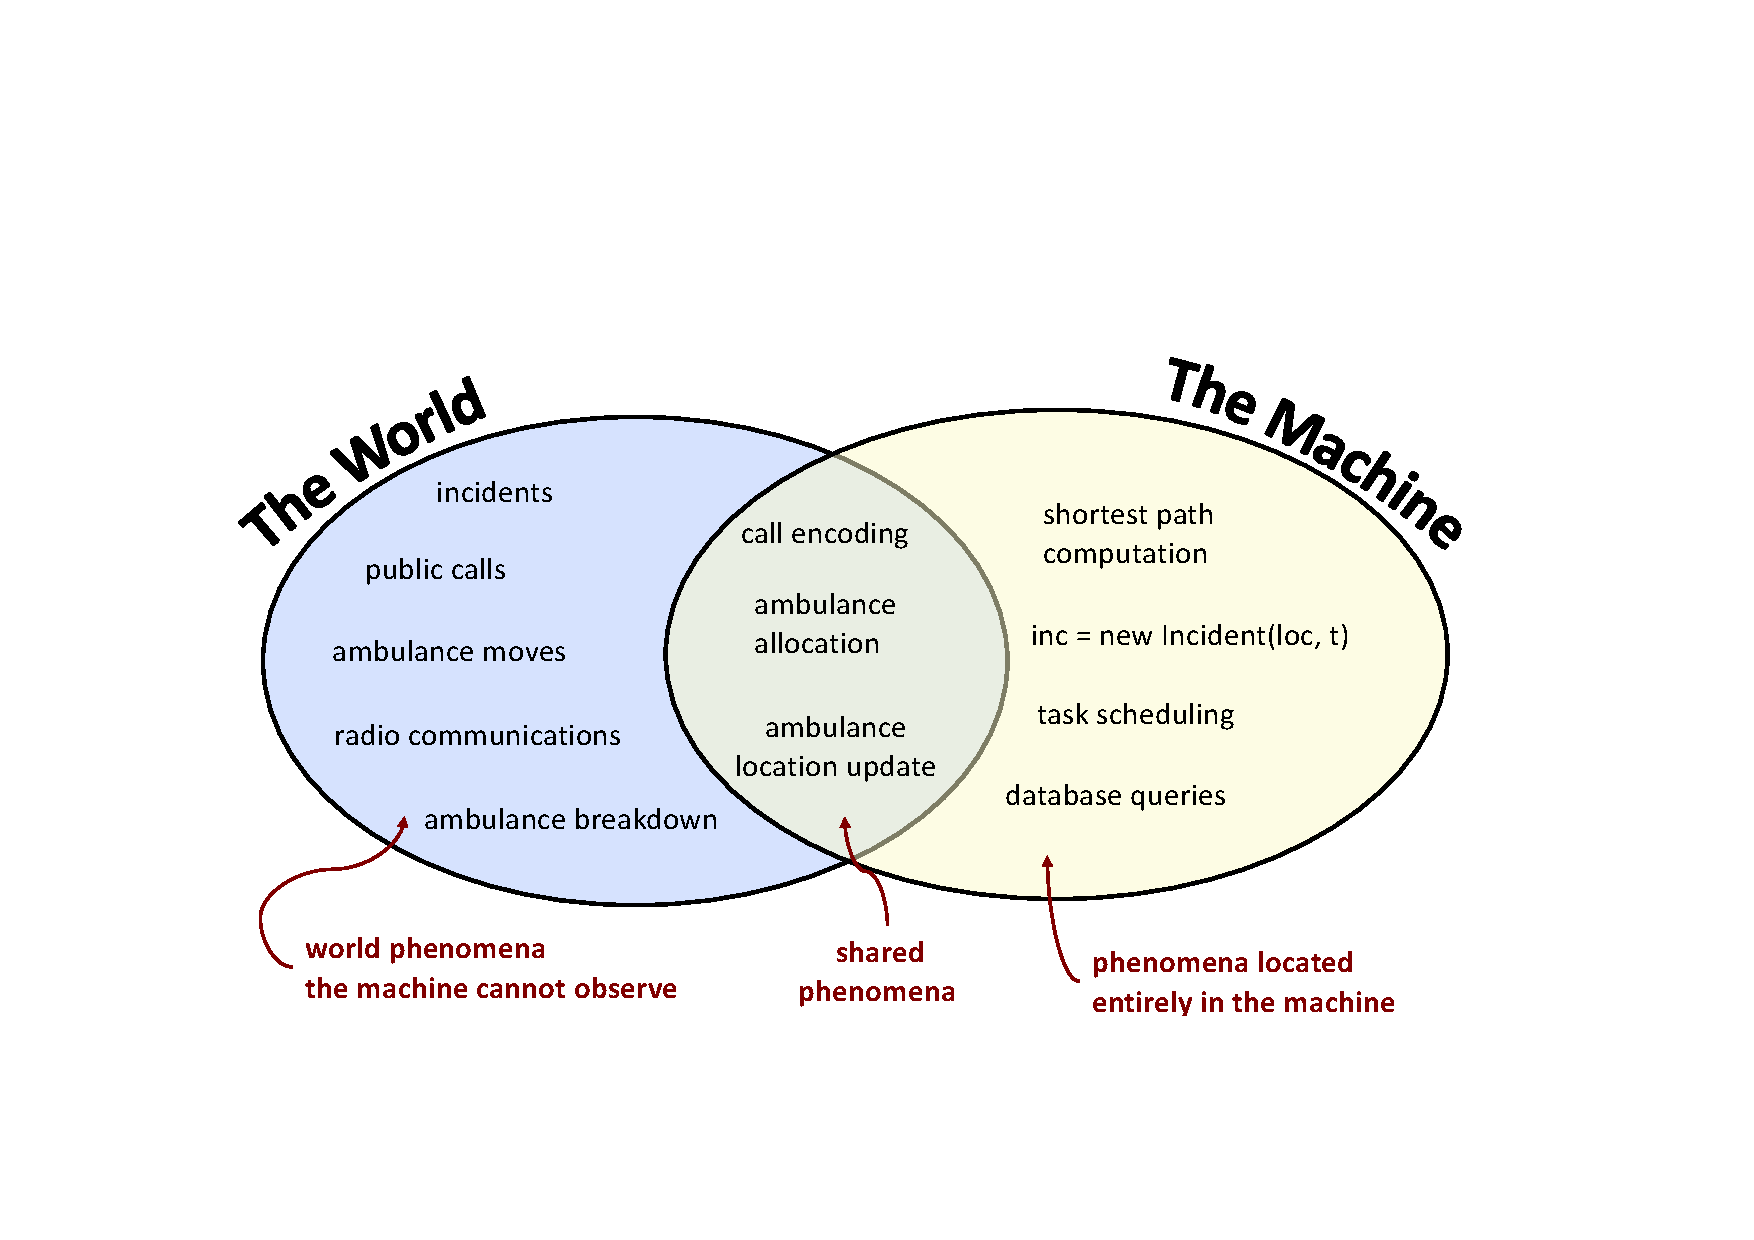
\includegraphics[width=\textwidth]{img/world-and-machine-1.pdf}
    \caption{The world and the machine sets, with reference to example on page~\pageref{example: ambulance dispatching system}.}
\end{figure}

\noindent
More generally, we can divide the machine and the world sets as:
\begin{itemize}
    \item The world which have goals and domain properties;
    \item The machine which have computers and programs;
    \item The requirements which is the bridge between the world and the machine.
\end{itemize}

\begin{figure}[!htp]
    \centering
    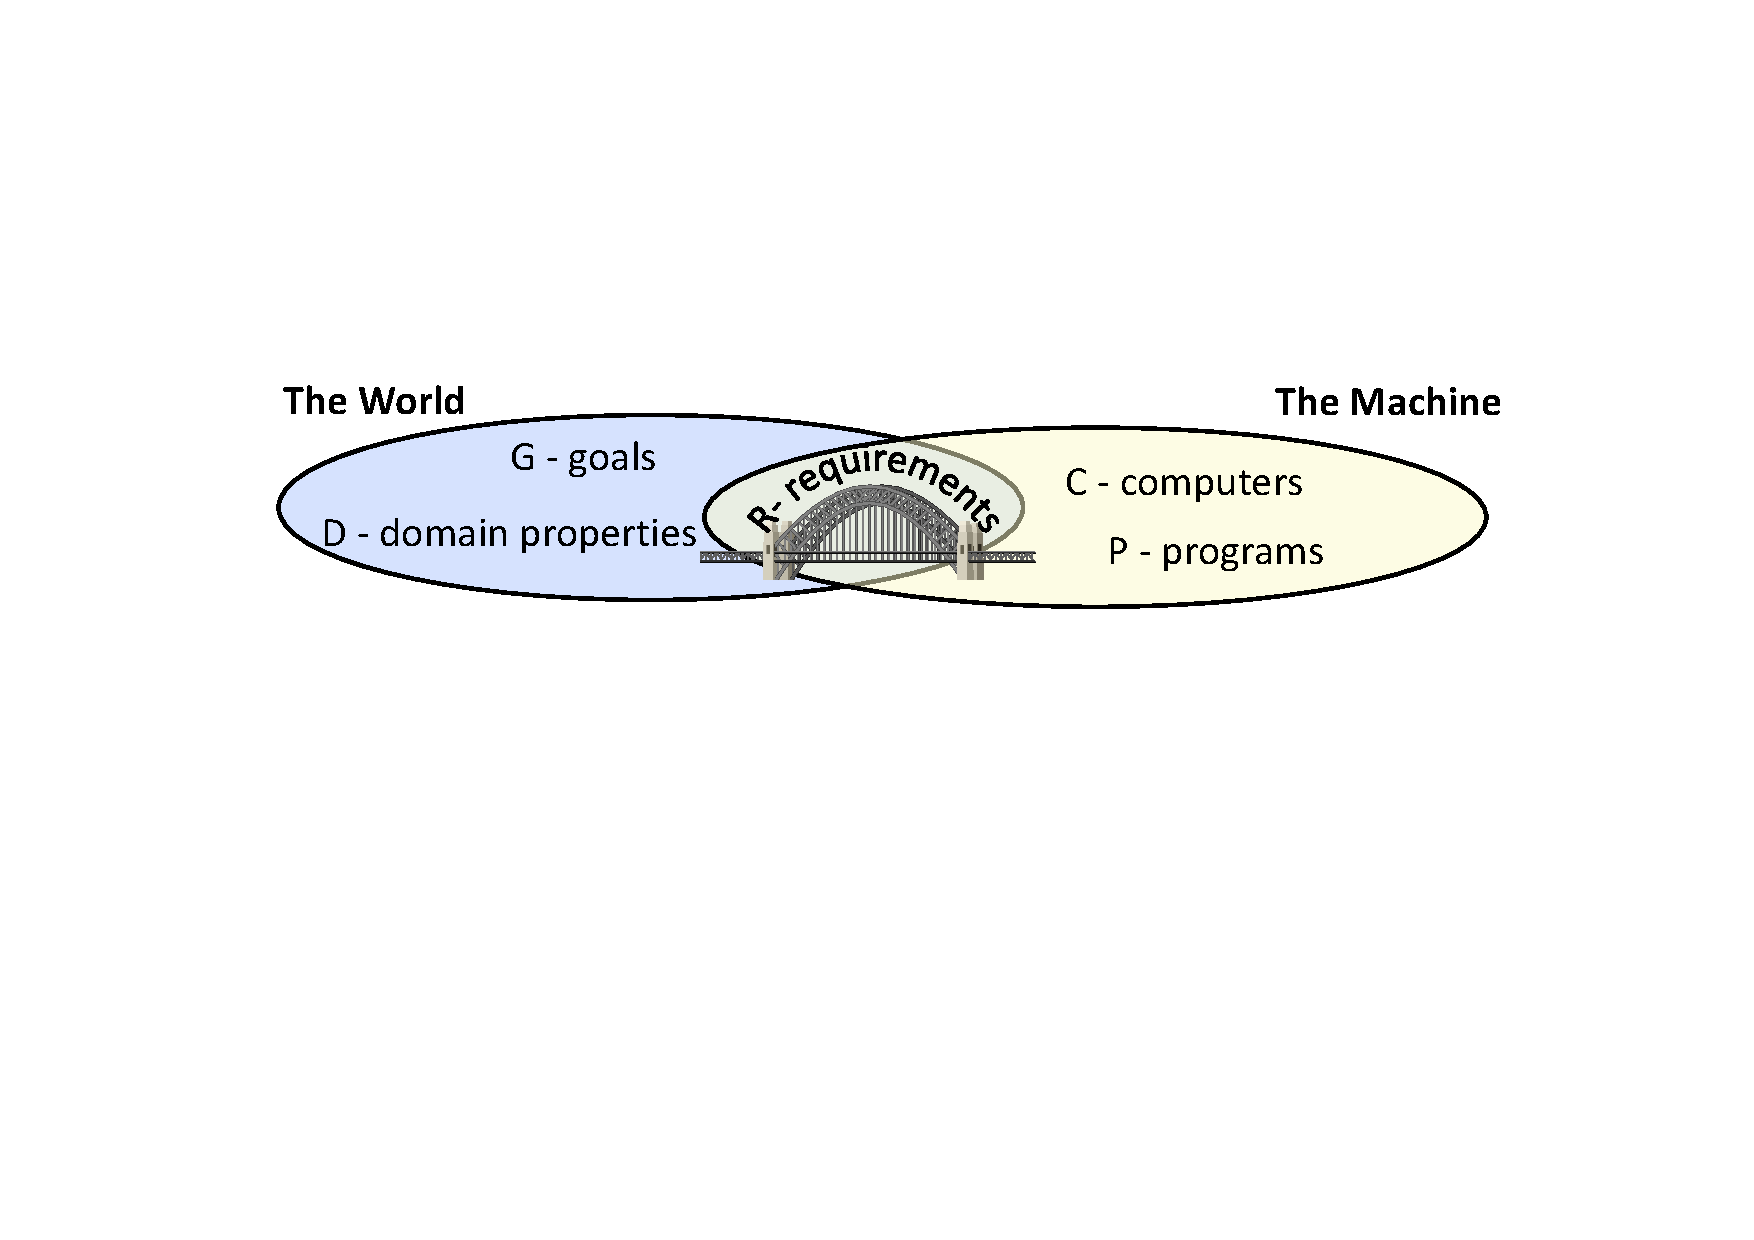
\includegraphics[width=\textwidth]{img/world-and-machine-2.pdf}
    \caption{Goals, domain properties, requirements, computers and programs.}
\end{figure}

\noindent
We explain more detailed these value inside the two sets:
\begin{itemize}
    \item \definition{Goals} are \textbf{prescriptive assertions formulated in terms of world phenomena} (not necessarily shared)
    \item \definition{Domain properties} (or assumptions) are \textbf{descriptive assertions assumed to hold in the world}
    \item \definition{Requirements} are \textbf{prescriptive assertions formulated in terms of shared phenomena} 
\end{itemize}

\newpage

\noindent
Using the \example{example} on the page~\pageref{example: ambulance dispatching system}, we can identify the goal, the domain assumptions and the requirement as follows:
\begin{itemize}
    \item \textbf{Goal}: \emph{For every urgent call reporting an incident, an ambulance should arrive at the incident scene within 14 minutes}.

    \item \textbf{Domain assumptions}:
    \begin{itemize}
        \item \emph{For every urgent call, details about the incident are correctly encoded}.
        \item \emph{When an ambulance is mobilized, it will reach the incident location in the shortest possible time}.
        \item \emph{Accurate ambulances' location are known by GPS}.
        \item \emph{Ambulance crews correctly signal ambulance availability through mobile data terminals on board of ambulances}.
    \end{itemize}
    
    \item \textbf{Requirement}: \emph{When a call reporting a new incident is encoded, the Automated Dispatching Software should mobilize the nearest available ambulance according to information available from the ambulances' GPS and mobile data terminals}.
\end{itemize}

\longline

\subsubsection{Completeness of Requirements}

Given the set of requirements \textbf{R}, goals \textbf{G} and domain assumptions \textbf{D}.

\begin{definitionbox}
    We say that \textbf{R} is \textbf{complete} \underline{if and only if}:
    \begin{itemize}
        \item \textbf{R} ensures satisfaction of \textbf{G} in the context of domain assumptions \textbf{D}
        \begin{center}
            \textbf{R and D $|=$ G}
        \end{center}
        We can make an analogy with program correctness. A program P running on a particular computer C is correct if it satisfies the requirement R: P and C $|=$ R.

        \item \textbf{G} captures all the \textbf{stakeholders' needs}.
        
        \item \textbf{D} represents \textbf{valid properties/assumptions about the world}.
    \end{itemize}
\end{definitionbox}